
\documentclass[border=5pt]{standalone}
\usepackage{amsmath}
\usepackage{pgfplots}
\pgfplotsset{compat=1.18}
\begin{document}
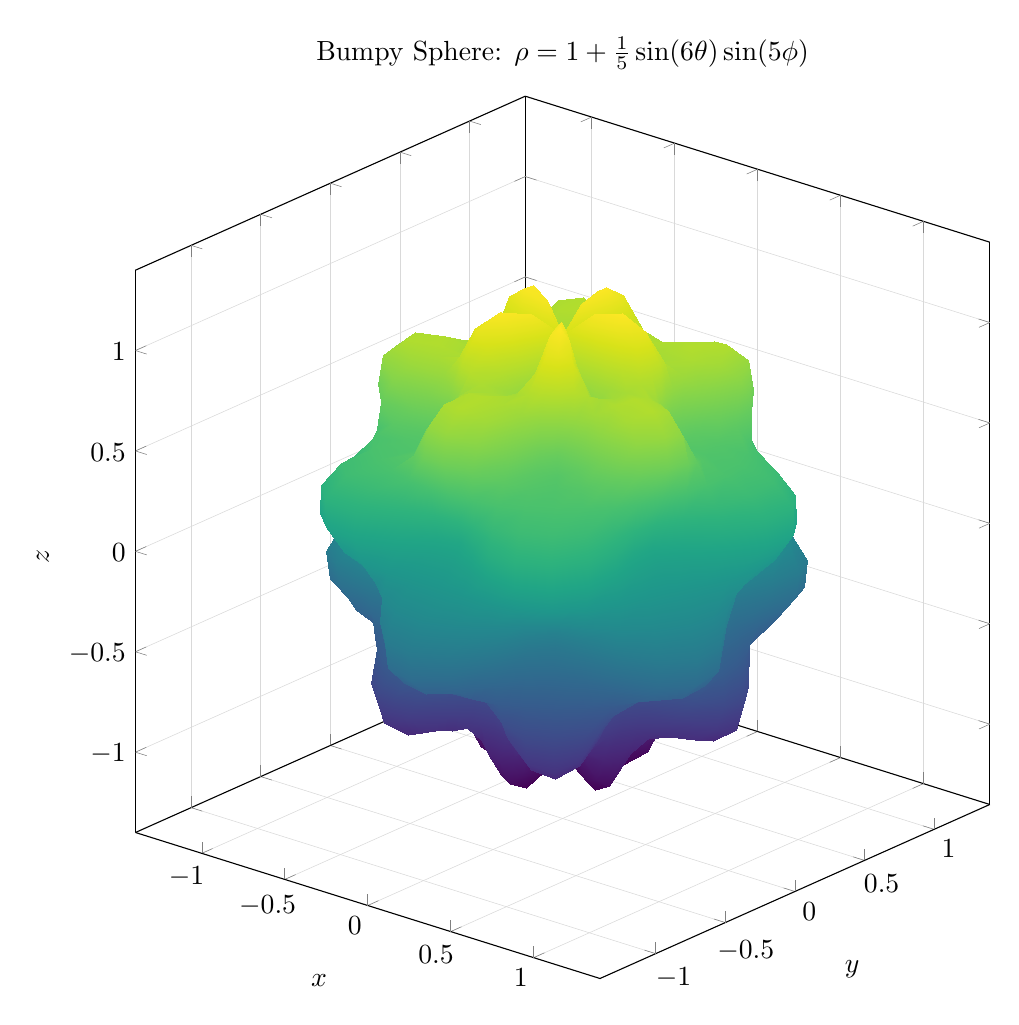
\begin{tikzpicture}
\begin{axis}[
    title={Bumpy Sphere: $\rho = 1 + \frac{1}{5}\sin(6\theta)\sin(5\phi)$},
    width=13cm, height=13cm,
    view={40}{22},
    xlabel={$x$}, ylabel={$y$}, zlabel={$z$},
    xmin=-1.4, xmax=1.4, ymin=-1.4, ymax=1.4, zmin=-1.4, zmax=1.4,
    enlargelimits=false,
    axis equal image,
    grid=major, grid style={very thin, gray!30},
    colormap/viridis,
    trig format plots=rad,
]
\addplot3[
    surf, shader=interp,
    samples=28, samples y=42,
    domain=0.02:3.14, y domain=0:6.2832,
    z buffer=sort,
] (
    {(1 + 0.2*sin(6*x)*sin(5*y)) * sin(x) * cos(y)},
    {(1 + 0.2*sin(6*x)*sin(5*y)) * sin(x) * sin(y)},
    {(1 + 0.2*sin(6*x)*sin(5*y)) * cos(x)}
);
\end{axis}
\end{tikzpicture}
\end{document}
